\thispagestyle{hoccungpinone}
\pagestyle{hoccungpi}
\everymath{\color{hoccungpi}}
\graphicspath{{../hoccungpi/pic/}}
\blfootnote{$^{1}$\color{hoccungpi}Đại học Bách Khoa Hà Nội.}
\begingroup
\AddToShipoutPicture*{\put(0,616){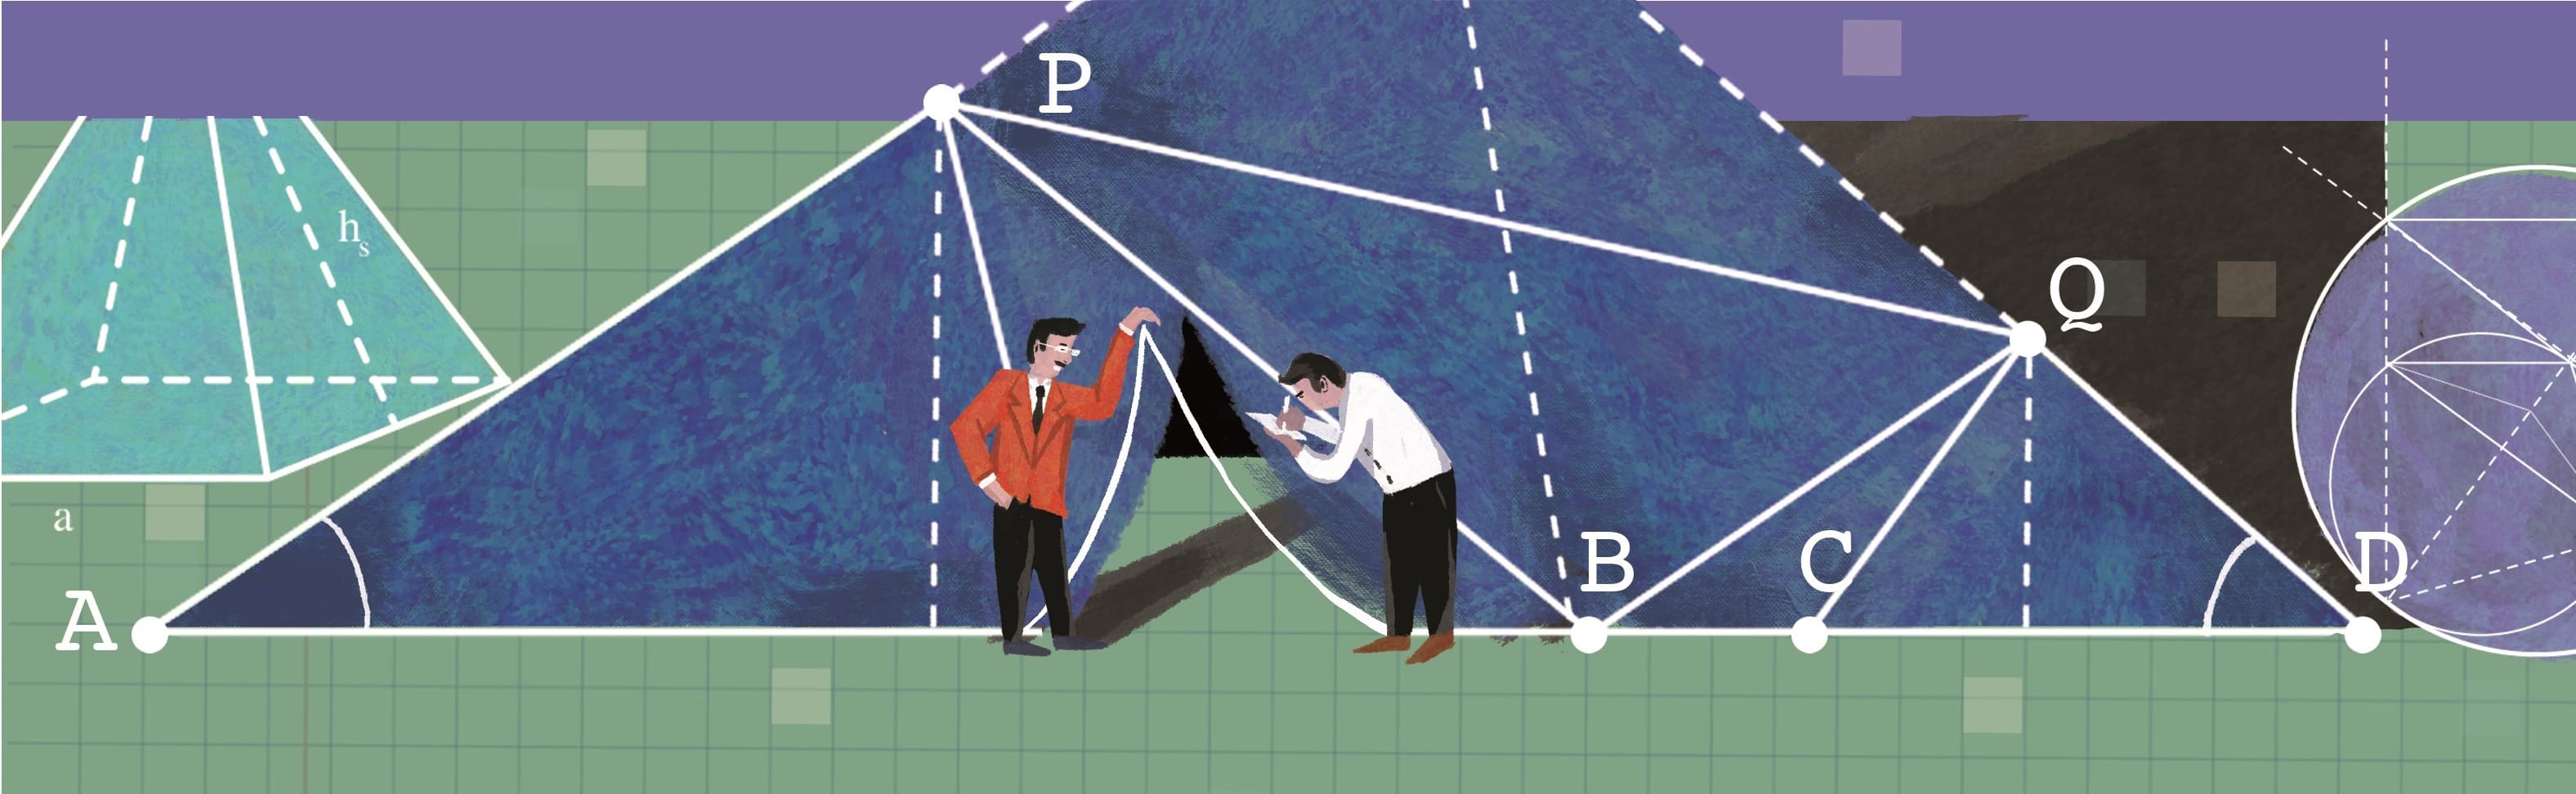
\includegraphics[width=19.3cm]{../bannerhoccungpi}}}
\AddToShipoutPicture*{\put(116,525){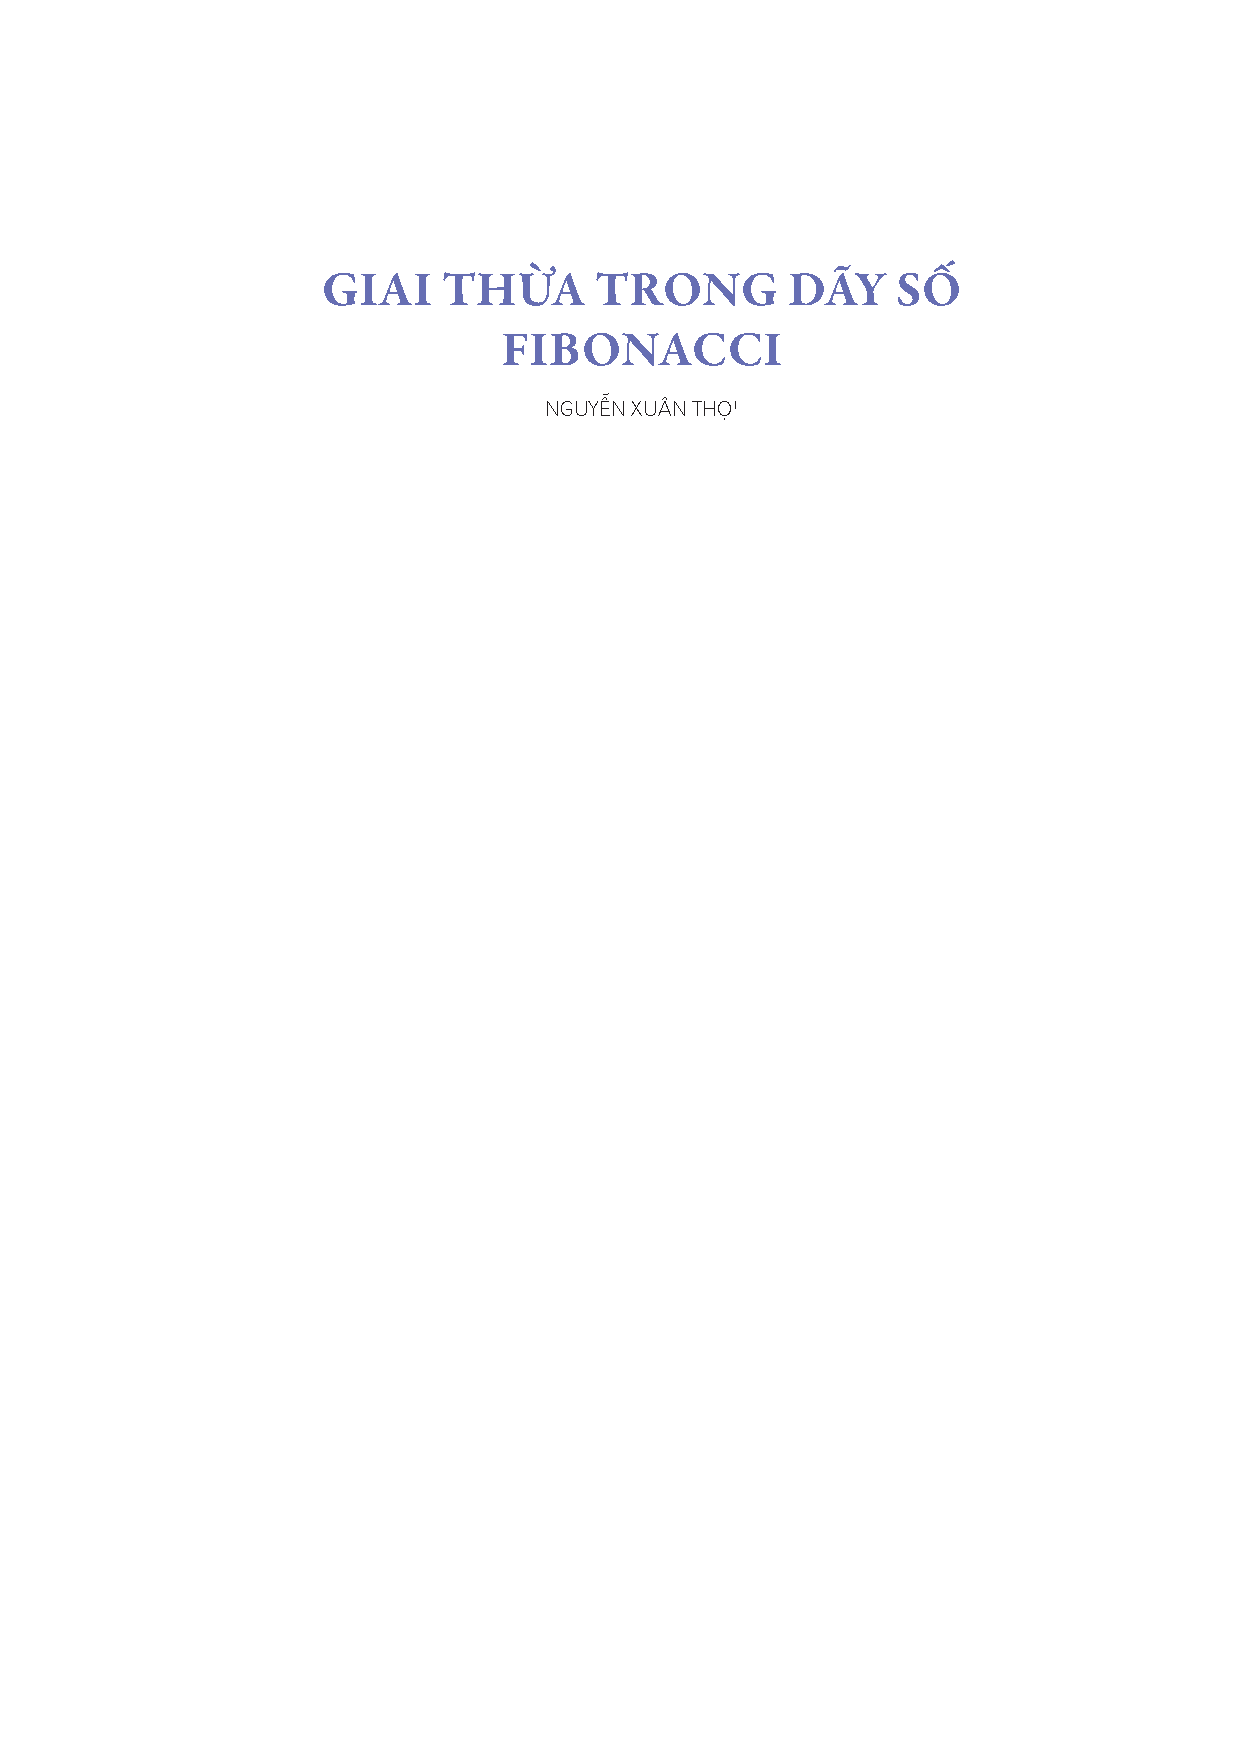
\includegraphics[scale=1]{../tieude.pdf}}}
\centering
\endgroup
\vspace*{185pt}

\begin{multicols}{2}
	Dãy số Fibonacci, đặt theo tên nhà toán học người Ý Fibonacci ($1170-1250$), được xác định bởi $F_0=0$, $F_1=1$, $F_{n+1}=F_n+F_{n-1}$ với mọi $n\geq 1$. 
	Đây là một trong những dãy số nổi tiếng nhất trong toán học. Tạp chí toán học Fibonacci Quaterly [$3$] của Canada chỉ xuất bản những nghiên cứu liên quan đến dãy Fibonacci. Vào năm $1964$, nhà toán học người Anh John H. E. Cohen chứng minh  có đúng ba số chính phương trong dãy Fibonacci, đó là $0$, $1$, và $144$ [$2$]. Một câu hỏi tự nhiên là liệu ta có thể tìm tất cả các giai thừa trong dãy Fibonacci. Câu hỏi này được giải quyết bởi Rajagopal và Griffiths [$5$]. Họ chỉ ra $1!$ và $2!$ là  hai số giai thừa duy nhất trong dãy Fibonacci. Nói cách khác, ta có định lý sau.
	\vskip 0.1cm
	\textbf{\color{hoccungpi}Định lý} $\pmb{1.}$ \textit{Phương trình
		\begin{align*}
			F_n=m! \tag{$1$}
		\end{align*}
		không có nghiệm nguyên dương với $n\ge 4$, trong đó $F_n$ là số Fibonacci thứ $n$. }
	\vskip 0.1cm
	Tuy nhiên, chứng minh của Rajagopal và Griffiths sử dụng định lý Carmichael về ước số nguyên thủy [$1$], một kết quả không tầm thường. Trong bài báo này, tác giả trình bày một chứng minh khác cho Định lý $1$. Với mỗi số nguyên dương $m$, ta ký hiệu $v_2(m)$ là số mũ cao nhất của $2$ chia hết $m$. Chú ý rằng với mọi $n > 0$ thì
	\begin{align*}
		F_n=\dfrac{u^n-v^n}{u-v}> \dfrac{u^n-1}{\sqrt{5}},
	\end{align*}
	trong đó $u=(1+\sqrt{5})/2$ và $v=(1-\sqrt{5})/2$.
	\vskip 0.1cm	
	Ta cần một số bổ đề.
	\vskip 0.1cm
	\textbf{\color{hoccungpi}Bổ đề} $\pmb{2}.$
	\textit{Với mọi số nguyên dương $n$ thì}
		\begin{align*}
			v_2(F_n)=
			\begin{cases}
				0 \text{ nếu } n\not\equiv 0 \,\,(\!\bmod{3})\\
				1 \text{ nếu } n\equiv 3 \,\,(\!\bmod{6}) \quad\quad\quad\text{\color{black}(}2\text{\color{black})}\\ 
				v_2(n)+2 \text{ nếu } n \equiv 0 \,\,(\!\bmod{6}).
			\end{cases} 
		\end{align*}
	Trong chứng minh Bổ đề [$2$], ta cần đến dãy số Lucas. Dãy Lucas $(L_n)_{n\geq 0}$ được xác định bởi  $L_0=2,\, L_1=1,\, L_{n+1}=L_n+L_{n-1}$ với mọi $n\geq 1$. Chú ý rằng $L_n=u^n+v^n$ với mọi $n\geq 0$.
	\vskip 0.1cm
	\textit{Chứng minh.} Xét dãy $(F_n)_{n\geq 0}$ modulo $4$: $0$, $1$, $1$, $2$, $3$, $1$, $0$, $1$, $1$, $2$, $3$, $...$ Đây là một dãy tuần hoàn theo chu kỳ $6$. Dễ thấy ($2$) đúng với $n\leq 6$. Giả sử ($2$) đúng với $n<k$ ($k\geq 6$, $k\in \mathbb{Z}^{+}$). Xét $n=k$. 
	Ta chỉ cần xét trường hợp $6\mid k$ vì nếu không $v_2(F_k)=0$ khi $3\nmid k$ và $v_2(F_k)=1$ khi $6\mid (k-3)$.
	\vskip 0.1cm	
	Đặt $k=6m$, với $m\in \mathbb{Z}^{+}$. Khi đó 
	\begin{align*}
			F_n&=\dfrac{u^{6m}-v^{6m}}{u-v}=\dfrac{u^{3m}-v^{3m}}{u-v}(u^{3m}+v^{3m})\\
			&=F_{3m}L_{3m}. \tag{$3$}
	\end{align*}
	Xét dãy $(L_n)_{n\geq 0}$  modulo $8$, dãy này có dạng:
		$2$, $1$, $3$, $4$, $7$, $3$, $2$, $5$, $7$, $4$, $3$, $7$, $2$, $1$, $3$, $...$
		Từ đó suy ra dãy Lucas modulo $8$ tuần hoàn với chu kỳ $12$. Hơn nữa, $8\nmid L_n$ với mọi $n\in \mathbb{Z}^{+}$ và 
		\begin{align*}
			v_2(L_n)=\begin{cases}
				0 \text{ nếu } n\equiv 1,2 \,\,(\!\bmod{3})\\
				2 \text{ nếu } n\equiv 3 \,\,(\!\bmod{6}) \quad\quad\quad \text{\color{black}(}4\text{\color{black})}\\ 
				1 \text{ nếu } n\equiv 0 \,\,(\!\bmod{6}).
			\end{cases} 
		\end{align*}
		Nếu $2\nmid m$ thì $3m\equiv 3 \pmod {6}$. Theo ($4$) thì $v_2(L_{3m})=2$. Từ ($3$) suy ra
		\begin{align*}
			v_2(F_{6m})=v_2(F_{3m})+2=3.
		\end{align*}
		Nếu $2|m$ thì $3m\equiv 0 \pmod {6}$. Theo ($4$)
		thì $v_2(L_{6m})=1$. Từ ($4$) suy ra
		\begin{align*}
			v_2(F_{6m})=v_2(F_{3m})+1=v_2(m)+3.
		\end{align*}
		Suy ra ($2$) đúng với $n=k+1$. Bổ đề được chứng minh. \hfill $\square$
	\vskip 0.1cm
	\textbf{\color{hoccungpi}Bổ đề} $\pmb{3.}$ \textit{Với mọi số nguyên dương {$n$} thì} 
		\begin{align*}
			v_2(n!)\geq n-1-\log_2 n.\tag{$5$}
		\end{align*}
	\textit{Chứng minh.}
	Giả sử $n$ có biểu diễn theo hệ nhị phân là
	\begin{align*}
		\overline{{s_ks_{k-1}}\ldots s_1}_{(2)}=n.
	\end{align*}
	Khi đó $s_k=1$ và $n\geq 2^{k-1}$.
	Đặt $S_2(n)=s_1+s_2+\cdots+s_k$.
	Thì
	\begin{align*}
		S_2(n)\leq k \leq 1+ \log_2 n.
	\end{align*}
	Mặt khác theo công thức Legendre\footnote[2]{\color{hoccungpi}Công thức Legendre nói rằng với mọi số nguyên tố $p$ thì $v_p(n!)=(n-S_p(n))/(p-1)$, trong đó $S_p(n)$ là tổng các chữ số trong biểu diễn cơ số $p$ của $n$.}   thì
	\begin{align*}
		v_2(n!)=n-S_2(n).
	\end{align*}
	Nên 
	\begin{align*}
	\quad\quad\quad	v_2(n!)\geq n-1-\log_2 n. \,\,\,\,\quad\quad\quad \square
	\end{align*}
	\textbf{\color{hoccungpi}Bổ đề} $\pmb{4.}$
	\textit{Với mọi số nguyên dương $n\geq 15$ thì}
		\begin{align*}
			2^{n-3}>n^3. \tag{$6$}
		\end{align*}
	\textit{Chứng minh.}
		Với $n=15$ thì ($6$) đúng vì $2^{12}=4096>3375=15^3$. Giả sử ($6$) đúng với $n=m\geq 15$. Khi đó 
		\begin{align*}
			2^{m+1-3} &=2\cdot 2^{m-3}>2m^3=m^3+m^3\\
			&\ge m^3+ 15m^2 = m^3 +\! 3m^2 \!+\! 3m +\! 1\\
			&\quad +3 (m^2-m)+ (m^2-1)+ 8m^2 \\
			&> m^3+3m^2+3m+1=(m+1)^3.
		\end{align*}
		Suy ra ($6$) đúng với $n=m+1$. Theo quy nạp có ($6$) đúng với mọi $n\geq 15$. \hfill $\square$
	\vskip 0.1cm
	\textbf{\color{hoccungpi}Bổ đề} $\pmb{5.}$
	\textit{Với mọi số nguyên dương $n\geq 2$ thì 
		\begin{align*}
			u^{n^2}>1+\sqrt{5}n!, \tag{$7$}
		\end{align*}
		trong đó $u=(1+\sqrt{5})/2$. }
	\vskip 0.1cm
	\textit{Chứng minh.} 
	Với $n=2$ thì ($7$) trở thành $u^4> 1+ 2\sqrt{5}$, hay $\frac{7+3\sqrt{5}}{2}> 1+ 2\sqrt{5}$, hay, một cách tương đương, $5> \sqrt{5}$, do đó hiển nhiên đúng. 
	\vskip 0.1cm	
	Giả sử ($7$) đúng với $n=m\geq 2$. Trước hết, để ý rằng $u^2 = \frac{3+ \sqrt{5}}{2}>2$, nói riêng $u^{2m}> 2^m= (1+1)^m = 1+ \binom{m}{1} + \cdots > m+1$ với mọi $m\ge 2$. Từ đó,
	\begin{align*}
			u^{(m+1)^2}&=u^{m^2}\cdot u^{2m+1}\\
			&> u^{m^2}\cdot u^{2m}\\
			&>(1+\sqrt{5}m!)(m+1)\\
			&>1+\sqrt{5}(m+1)!.
	\end{align*}
	Suy ra ($7$) đúng với $n=m+1$. Như vậy, theo nguyên lý quy nạp thì ($7$) đúng với mọi \linebreak $n\geq 2$.\hfill $\square$
	\vskip 0.1cm
	Bây giờ ta chứng minh Định lý $1$.
	\vskip 0.1cm
	\textit{Chứng minh.}
	Giả sử tồn tại các số nguyên dương $m,n$ với $n\geq 4$ sao cho
	\begin{align*}
			F_n=m!. \tag{$8$}
	\end{align*}
	Do $F_4=3$ không là một số giai thừa nên ta phải có $F_n\geq F_5 =5$, dẫn đến $m\geq 3$. Nếu $m=4$ thì $F_n=24$, điều này là vô lý do dãy Fibonacci là dãy số tăng kể từ số hạng thứ ba và $F_8=21< 24< F_9=34$. Suy ra $m\geq 5$. Khi đó $3,4,5$ đều là ước của $m!$ nên cũng là ước của $F_n$. Theo ($2$) ta có $6\mid n$. 
	\vskip 0.1cm	
	Xét dãy $(F_n)_{n\geq 0}$  modulo $3$: $0$, $1$, $1$, $2$, $0$, $2$, $2$, $1$, $0$, $1$, $1$, $...$ Từ đó suy ra dãy Fobonacci modulo $3$ tuần hoàn với chu kỳ $8$ và $3\mid F_n$ khi và chỉ khi $4\mid n$.
	\vskip 0.1cm
	Xét dãy $(F_n)_{n\geq 0}$ modulo $5$:
	$0$, $1$, $1$, $2$, $3$, $0$, $3$, $3$, $1$, $4$, $0$, $4$, $4$, $3$, $2$, $0$, $2$, $2$, $4$, $1$, $0$, $1$, $1$, $...$
	Suy ra dãy Fibonacci modulo $5$ tuần hoàn với chu kỳ $20$ và $5\mid F_n$ khi và chỉ khi $5\mid n$. 
	\vskip 0.1cm	
	Từ các lập luận trên ta suy ra $4,5,6$ đều là ước của $n$. Suy ra $60\mid n$. Nói riêng, ta có $n\geq 60$. Chú ý rằng $u^2>2$ nên
	\begin{align*}
		m!=F_n\geq F_{60}>\dfrac{u^{60}-1}{\sqrt{5}}>15!.
	\end{align*}
	Trong ước lượng trên, bất đẳng thức $(u^{60}-1)/(15!\sqrt{5})>1$ có thể được kiểm tra bằng các tính toán trực tiếp dựa vào các phần mềm tính toán hoặc chỉ đơn giản bằng một chiếc máy tính cầm tay.
	Suy ra 
	\begin{align*}
		m\geq 16.
	\end{align*} 
	Nhắc lại rằng, theo ($2$) thì
	\begin{align*}
		v_2(F_n)=2+v_2(n).
	\end{align*}
	Kết hợp điều này với ($5$) ta suy ra 
	\begin{align*}
		2+v_2(n)= v_2(m!)\geq m-1-\log_2 m,
	\end{align*}
	cho nên 
	\begin{align*}
		v_2(n)\geq m-3-\log_2 m.
	\end{align*}
	Do đó, ta có 
	\begin{align*}
			n\geq 2^{v_2(n)}\geq  \dfrac{2^{m-3}}{m}. \tag{$9$}
	\end{align*}
	Chú ý rằng $m\geq 16$ nên bằng cách kết hợp ($6$), ($7$), và ($9$) ta thu được
	\begin{align*}
		m!=F_n&>\dfrac{u^n-1}{\sqrt{5}}>\dfrac{u^{2^{m-3}/{m}}-1}{\sqrt{5}}\\&>\dfrac{u^{m^2}-1}{\sqrt{5}}>m!,
	\end{align*}
	vô lý. Định lý $1$ được chứng minh. \hfill $\square$
	\vskip 0.1cm
	\textbf{\color{hoccungpi}Tài liệu tham khảo}
	\vskip 0.1cm
	[$1$] R. D. Carmichael, On the numerical factors of the arithmetic forms $\alpha^n\pm \beta^n$, Annals of Mathematics, $15$ ($1/4$) ($1913$), $30-70$.
	\vskip 0.1cm
	[$2$] J. H. E. Cohn, Square Fibonacci numbers, Fibonacci Quarterly, $2$ ($2$)
		($1964$), $109-113$.
	\vskip 0.1cm
	[$3$] Fibonacci Quaterly. \url{https://www.fq.math.ca/}
	\vskip 0.1cm
	[$4$] Legendre's formula, Wikipedia. \url{https://en.wikipedia.org/wiki/Legendre%27s_formula}
	\vskip 0.1cm
	[$5$] S.~Rajagopal và M.~Griffiths,  On Fibonacci numbers that are factorials, Mathematical Gazette, {$98$} ($541$) (March $2014$), $104-107$.
\end{multicols}